\documentclass[11pt]{article}
\usepackage[margin=1in]{geometry}
\usepackage{amsmath,amssymb,booktabs,graphicx,setspace,caption,hyperref}
\usepackage[T1]{fontenc}
\usepackage{mathpazo}
\setlength{\parindent}{0pt}
\setlength{\parskip}{0.6em}
\captionsetup{font=small,skip=6pt}
\title{Panel MS-AR(1): common trend vs Pareto random intercepts\\[0.4em]\large Quarterly dummies, real GDP per worker}
\author{}
\date{}
\begin{document}
\maketitle
\section{Model}
Joint panel Markov-switching AR(1) around a linear trend with common quarterly dummies (Q1 omitted):
\begin{align}
y_{it} &= a_i + g\, t + d_2 Q2_t + d_3 Q3_t + d_4 Q4_t + z_{it}, \\
z_{i,t+1} &= \bigl(1-\rho(s_{it})\bigr)\mu(s_{it}) + \rho(s_{it})\, z_{it} + \sigma(s_{it})\,\varepsilon_{it}, \\
s_{i,t+1} &\sim \Pi(\,\cdot\mid s_{it}).
\end{align}
Specification 1 sets $a_i\equiv a$. Specification 2 draws $a_i$ from a shifted Type II Pareto (Lomax) on $[m,\infty)$, with location $m$, scale $\sigma$, and shape $\alpha$: $P(a_i>x)=(1+(x-m)/\sigma)^{-\alpha}$ for $x\ge m$. The country likelihood integrates $a_i$ by 15-point Gauss--Legendre on the probability-integral-transform scale. The slope $g$ and the quarterly dummies are common. $|\rho|<0.99$. Median $\mu$ pinned at 0. Cycles use posterior-mean $a_i$. Standard errors are delta-method from a numerical Hessian.
\clearpage
\section{Common intercept, linear trend, and quarterly dummies}
2026-09-14 panel, full sample: log real GDP per worker. 90 countries, 8489 observations, 1963-Q1--2026-Q2. Fitted countries: 90. Observations: 8489. Log-likelihood: 13182.75. Ergodic mean of the cycle $E[z]=0.5738$ (0.0863).
Common intercept $a=-5.4283$ (0.1150). Common slope $g=-0.0004$ (0.0016). Seasonal dummies (Q1 omitted): $d_{Q2}=0.0161$ (0.0008), $d_{Q3}=0.0106$ (0.0009), $d_{Q4}=0.0432$ (0.0008).
\begin{table}[h]
\centering
\caption{Regime AR(1), transition matrix, and ergodic $\pi$. Columns are regimes.}
\begin{tabular}{lccc}
\toprule
 & (0) & (1) & (2) \\
\midrule
$\mu$ & -0.8032 & 0.0000 & 1.4857 \\
 & (0.3159) & --- & (0.0734) \\ \addlinespace
$\sigma$ & 0.1789 & 0.0660 & 0.0281 \\
 & (0.0049) & (0.0012) & (0.0004) \\ \addlinespace
$\rho$ & 0.9900 & 0.9900 & 0.9900 \\
 &  & (0.0000) & (0.0000) \\ \addlinespace
$\Pi_{0\cdot}$ & 0.9786 & 0.0171 & 0.0042 \\
 & (0.0060) & (0.0050) & (0.0030) \\ \addlinespace
$\Pi_{1\cdot}$ & 0.0040 & 0.9812 & 0.0148 \\
 & (0.0013) & (0.0028) & (0.0025) \\ \addlinespace
$\Pi_{2\cdot}$ & 0.0016 & 0.0138 & 0.9846 \\
 & (0.0012) & (0.0023) & (0.0021) \\ \addlinespace
$\pi$ & 0.1159 & 0.4351 & 0.4490 \\
 & (0.0248) & (0.0346) & (0.0362) \\ \addlinespace
\bottomrule
\end{tabular}
\end{table}
\begin{figure}[h]
\centering
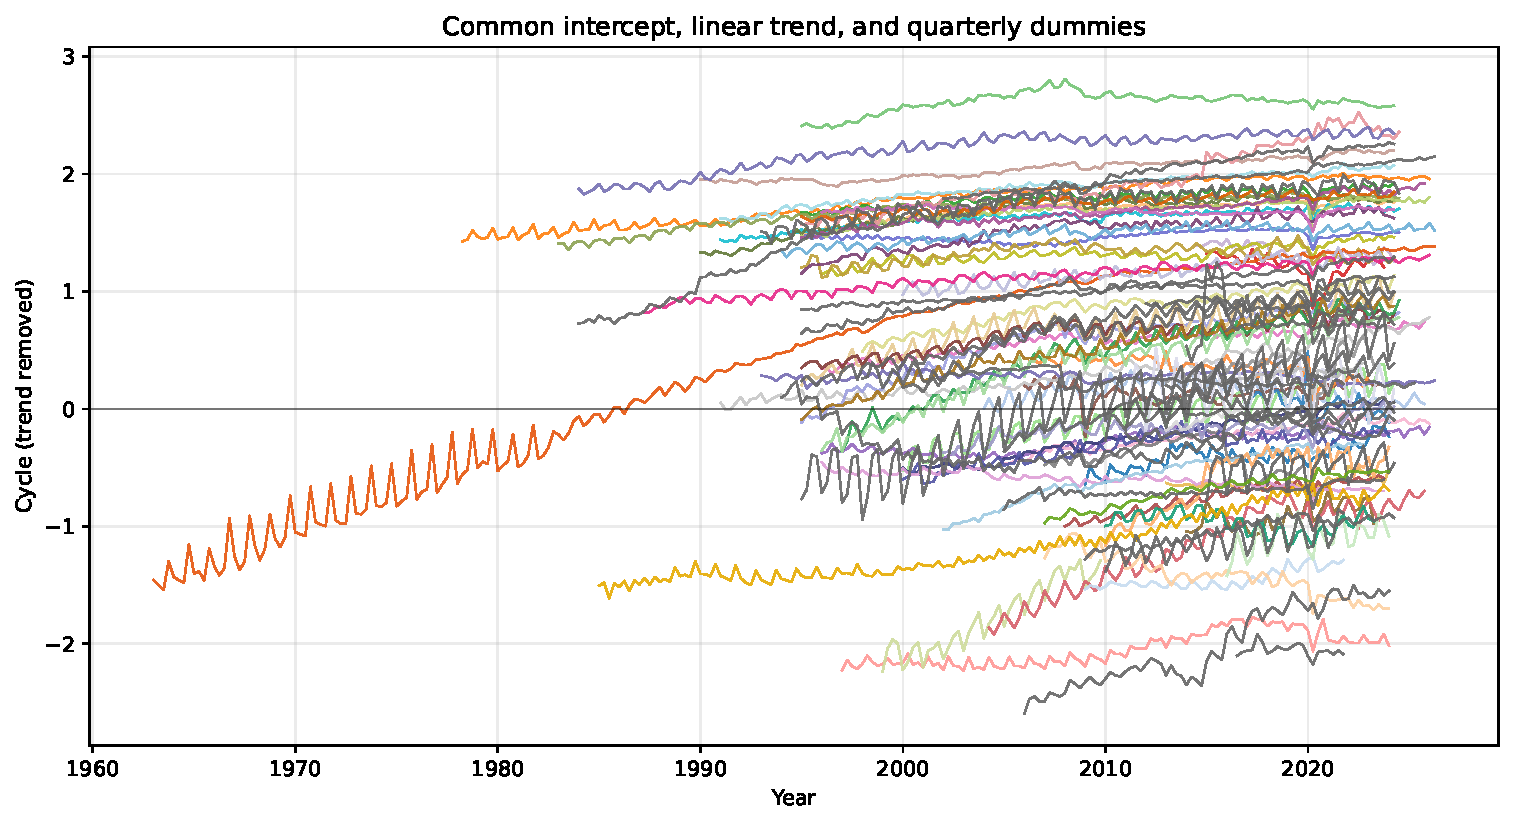
\includegraphics[width=0.75\textwidth]{figs/cycle_common_ag_q.pdf}
\caption{Country cycles after removing the linear trend and quarterly means.}
\end{figure}
\clearpage
\section{Pareto RE intercepts, common trend and quarterly dummies}
2026-09-14 panel, full sample: log real GDP per worker. 90 countries, 8489 observations, 1963-Q1--2026-Q2. Fitted countries: 90. Observations: 8489. Log-likelihood: 13439.80. Ergodic mean of the cycle $E[z]=0.1664$ (0.0756).
Random intercepts Type II Pareto on $[m,\infty)$ with location $m=-7.4177$ (0.1116), scale $=16.4022$ (6.2334), shape $\alpha=19.5016$ (6.8641). Posterior-mean $a_i$: mean -6.145, min -7.393, max -4.231. Common slope $g=0.0167$ (0.0012). Seasonal dummies (Q1 omitted): $d_{Q2}=0.0164$ (0.0008), $d_{Q3}=0.0107$ (0.0009), $d_{Q4}=0.0423$ (0.0008).
\begin{table}[h]
\centering
\caption{Regime AR(1), transition matrix, and ergodic $\pi$. Columns are regimes.}
\begin{tabular}{lccc}
\toprule
 & (0) & (1) & (2) \\
\midrule
$\mu$ & -0.2856 & 0.0000 & 0.6033 \\
 & (0.1012) & --- & (0.1080) \\ \addlinespace
$\sigma$ & 0.1678 & 0.0653 & 0.0266 \\
 & (0.0047) & (0.0011) & (0.0004) \\ \addlinespace
$\rho$ & 0.6946 & 0.9900 & 0.9900 \\
 & (0.0339) & (0.0001) & (0.0000) \\ \addlinespace
$\Pi_{0\cdot}$ & 0.9833 & 0.0083 & 0.0083 \\
 & (0.0048) & (0.0038) & (0.0038) \\ \addlinespace
$\Pi_{1\cdot}$ & 0.0029 & 0.9837 & 0.0134 \\
 & (0.0009) & (0.0026) & (0.0025) \\ \addlinespace
$\Pi_{2\cdot}$ & 0.0014 & 0.0126 & 0.9860 \\
 & (0.0007) & (0.0020) & (0.0020) \\ \addlinespace
$\pi$ & 0.1128 & 0.4188 & 0.4684 \\
 & (0.0256) & (0.0366) & (0.0373) \\ \addlinespace
\bottomrule
\end{tabular}
\end{table}
\begin{figure}[h]
\centering
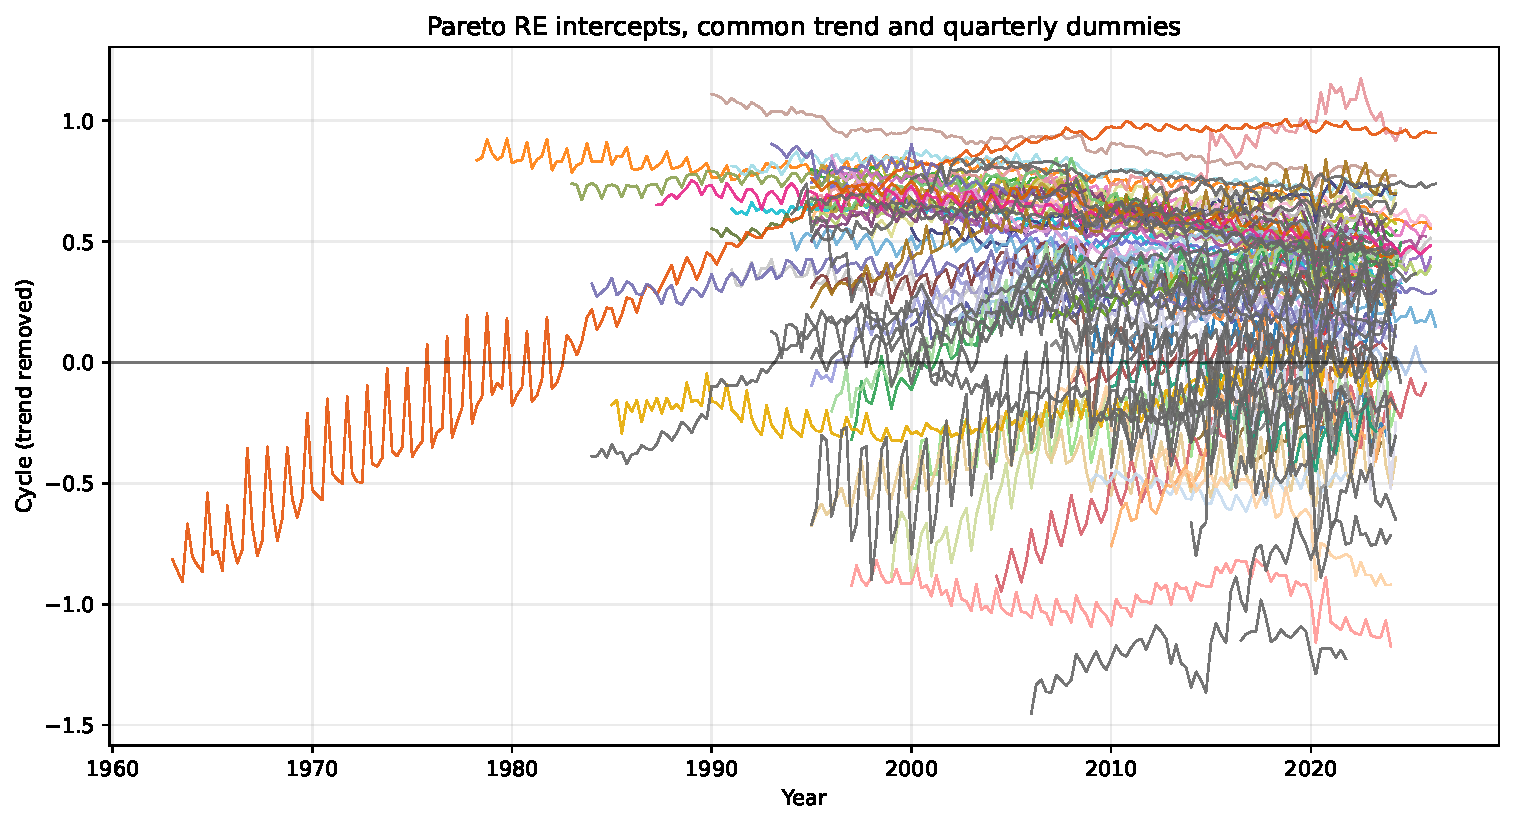
\includegraphics[width=0.75\textwidth]{figs/cycle_pareto_ai_q.pdf}
\caption{Country cycles after removing the linear trend and quarterly means.}
\end{figure}
\end{document}
